\section{Pezzi utili di \LaTeX{}}

\subsection{Template vari}

\begin{algorithm}[H]
\caption{Divide and Conquer}\label{alg:dnc}
\begin{algorithmic}[1]
    \Procedure{Divide\&Conquer}{$i$}
        \If{$|i| \leq n_0$}
        \Comment{BASE}
            \State *risolvo direttamente*
        \EndIf
        \State $\langle i_1, i_2, \dots, i_k \rangle \gets A_D(i)$ 
        \Comment{DIVIDE}
        \For{$j \gets 1 $ to $ k $ }
        \Comment{RECURSE}
            \State $s_j \gets
            \Call{Divide\&Conquer}{i_j}
            $
        \EndFor
        \State $s \gets A_C(\langle s_1, s_2, \dots, s_k \rangle)$
        \Comment{CONQUER}
        \State return $s$
    \EndProcedure
\end{algorithmic}
\end{algorithm}
\noindent
Testo non identato!
\begin{algorithm}[H]
\caption{Esempi in libertà}\label{alg:esempi}
\begin{algorithmic}[1]
    \Procedure{Esempi}{$n$}
        \If{$|i| \leq n_0$}
        \Comment{if}
            \State *risolvo direttamente*
        \EndIf
        \ForAll{$i \in A_n$}
        \Comment{for each}
            \State $s \gets
            \Call{Magic}{i}
            $
        \EndFor
        \RepLoop{$k$}
        \Comment{repeat some times}
            \State $t \gets \Call{Full\_Contraction}{\bgg{}} $
            \State $min \gets \Call{Min}{min, t} $
        \EndRepLoop
        \State \Return $x$
        \Comment{il return che vorrei}
    \EndProcedure
    \Function{Unbias}{ }
        \Comment{funzioni}
        \State \Return $0$
    \EndFunction
\end{algorithmic}
\end{algorithm}

\begin{definition}[Algoritmo]\label{def:algex}
    Un algoritmo è una procedura computazionale finita (terminante) e deterministica, specificata come una sequenza di passi elementari (istruzioni) estratte da un insieme standard associato a un modello computazionale (astrazione di un computer) che trasforma in maniera univoca un ingresso in un uscita.
\end{definition}

Guarda che so fare
\begin{align*}
    &
    \setzo{m}
    \quad
    \setzo{}
    \quad
    \odot
    \quad
    \oplus
    \quad
    \zz{n}
    \quad
    \zs
    \quad
    \zs{\rho(n)}
    \quad
    \equiv_n
    \\
    &
    \ldblbrace
        u = 1
    \rdblbrace
    \ldblbraceb
        u = 1
    \rdblbraceb
    \ldblbraceB
        u = 1
    \rdblbraceB
    \ldblbracebb
        u = 1
    \rdblbracebb
    \ldblbraceBB
        u = 1
    \rdblbraceBB
    \\
    &
    \ldblbrace
        \left\{ x, y \right\}
        :
        \left( x = u \right)
        \vee
        \left( y = v \right)
    \rdblbrace
\end{align*}

Un problema
\begin{align*}
    SS: & \\
    \texttt{istanza:} \quad &
    \langle
        S,t
    \rangle
    \\
    \text{dove} \quad &
    S \subseteq \mathbb{N} - \left\{ 0 \right\} \text{ finito}
    \\
    &
    t \subseteq \mathbb{N} - \left\{ 0 \right\} \\
    \texttt{domanda:} \quad &
    \exists \, S' \subseteq S : \sum_{s \in S'}^{} s = t \, ?
\end{align*}

Una lista
\begin{itemize}[noitemsep,parsep=0pt,partopsep=0pt,topsep=0pt]
    \item[--] $L_A = L$ (il linguaggio deciso da $A$ è $L$)
    \item[--] $T_A(|x|) = O(|x|^k)$ per qualche costante $k \geq 0$
\end{itemize}

Una tabella con spazi aggiunti \url{https://tex.stackexchange.com/a/65128}
\begin{equation*}
    \begin{array}[h]{cc|c}
        x & y & \text{prob} \\
        \hline
        \rule{0pt}{1.0\normalbaselineskip}
        0 & 0 & (1-p)^2 \\
        0 & 1 & p(1-p) \\
        1 & 0 & p(1-p) \\
        1 & 1 & p^2
    \end{array}
\end{equation*}

\subsection{Teoremi e vari ambienti }

\begin{theorem}
    Un teorema senza nome
\end{theorem}

\begin{corollario}
    Un primo corollario
\end{corollario}

\begin{corollario}
    Un secondo corollario
\end{corollario}

\begin{theorem}[Nome del teorema]
    Un teorema con nome
\end{theorem}

\begin{corollario}
    Un primo corollario del teorema con nome
\end{corollario}

\begin{definition}
    Una definizione utile, la seconda di questa sezione
\end{definition}

\begin{proposizione}[Nome della proposizione]
    Una proposizione con nome
\end{proposizione}

\begin{corollario}
    Un primo corollario della proposizione con nome
\end{corollario}

\subsection{Grafi}

Grafi facili da mantenere

% Declare layers (done in main)
\pgfdeclarelayer{background}
\pgfsetlayers{background,main}

\begin{figure}[h]
    \centering
    \caption{Algoritmo di Prim}
    \label{fig:prim1}
    %%%%%%%%%%%%%%%%%%%%%%%%%%%%%%%%%%%%%%%%%%%%%%%%%%%%%%%%%%%%%%%%%%%%%%%%%%%%%%%%%%%%%
    \begin{subfigure}[b]{0.45\textwidth}
        \centering
        \caption{Archi uscenti dal primo nodo}
        \label{fig:au1}
        \begin{tikzpicture} [
                % automagically put labels not on edges
                auto,
                % exchanges the roles of left and right in automatic placement
                % the side the label is put on depends on the order of the nodes in the edge
                swap,
                scale=1.4,
                vertex/.style={circle,fill=black!25,minimum size=20pt,inner sep=0pt},
                selected vertex/.style = {vertex, fill=red!24},
                edge/.style = {draw,thick,-},
                weight/.style = {font=\small},
                selected edge/.style = {draw,line width=5pt,-,red!50},
                outbound edge/.style = {draw,line width=5pt,-,blue!50},
                ignored edge/.style = {draw,line width=5pt,-,black!20}
            ]
            % First we draw the vertices
            \foreach \pos/\name in {
                {(0,0)/d}, {(0,2)/a}, {(1.5,2)/b}, {(4,2)/c}, {(3,1.2)/e}, {(2,0)/f}, {(4,0)/g}}
                \node[vertex] (\name) at \pos {$\name$};
            % Connect vertices with edges and draw weights
            \foreach \source/ \dest /\weight in {b/a/7, c/b/8, d/a/5, d/b/9,
                                                 e/b/7, e/c/5, e/d/15,
                                                 f/d/6, f/e/8, g/e/9, g/f/11}
                \path[edge] (\source) -- node[weight] {$\weight$} (\dest);
            % color a node
            % \path node[selected vertex] at (d) {$d$};
            % prepare it in loop version anyway
            \foreach \vertex in {d}
                \path node[selected vertex] at (\vertex) {$\vertex$};
            % For convenience we use a background layer to highlight edges
            % This way we don't have to worry about the highlighting covering
            % weight labels. 
            \begin{pgfonlayer}{background}
                \foreach \source / \dest in {d/a,d/b,d/e,d/f}
                    \path[outbound edge] (\source.center) -- (\dest.center);
            \end{pgfonlayer}
        \end{tikzpicture}
    \end{subfigure}
    \quad
    %%%%%%%%%%%%%%%%%%%%%%%%%%%%%%%%%%%%%%%%%%%%%%%%%%%%%%%%%%%%%%%%%%%%%%%%%%%%%%%%%%%%%
    \begin{subfigure}[b]{0.45\textwidth}
        \centering
        \caption{Arco selezionato}
        \label{fig:au2}
        \begin{tikzpicture} [
                auto,
                swap,
                scale=1.4,
                vertex/.style={circle,fill=black!25,minimum size=20pt,inner sep=0pt},
                selected vertex/.style = {vertex, fill=red!24},
                edge/.style = {draw,thick,-},
                weight/.style = {font=\small},
                selected edge/.style = {draw,line width=5pt,-,red!50},
                outbound edge/.style = {draw,line width=5pt,-,blue!50},
                ignored edge/.style = {draw,line width=5pt,-,black!20}
            ]
            % First we draw the vertices
            \foreach \pos/\name in {
                {(0,0)/d}, {(0,2)/a}, {(1.5,2)/b}, {(4,2)/c}, {(3,1.2)/e}, {(2,0)/f}, {(4,0)/g}}
                \node[vertex] (\name) at \pos {$\name$};
            % Connect vertices with edges and draw weights
            \foreach \source/ \dest /\weight in {b/a/7, c/b/8, d/a/5, d/b/9,
                                                 e/b/7, e/c/5, e/d/15,
                                                 f/d/6, f/e/8, g/e/9, g/f/11}
                \path[edge] (\source) -- node[weight] {$\weight$} (\dest);
            % color a node
            \foreach \vertex in {d,a}
                \path node[selected vertex] at (\vertex) {$\vertex$};
            \begin{pgfonlayer}{background}
                \foreach \source / \dest in {b/a,d/b,d/e,d/f}
                    \path[outbound edge] (\source.center) -- (\dest.center);
                \foreach \source / \dest in {d/a}
                    \path[selected edge] (\source.center) -- (\dest.center);
            \end{pgfonlayer}
        \end{tikzpicture}
    \end{subfigure}
    \\[2pt]
    %%%%%%%%%%%%%%%%%%%%%%%%%%%%%%%%%%%%%%%%%%%%%%%%%%%%%%%%%%%%%%%%%%%%%%%%%%%%%%%%%%%%%
    \begin{subfigure}[b]{0.45\textwidth}
        \centering
        \caption{Secondo arco selezionato}
        \label{fig:au3}
        \begin{tikzpicture} [
                auto,
                swap,
                scale=1.4,
                vertex/.style={circle,fill=black!25,minimum size=20pt,inner sep=0pt},
                selected vertex/.style = {vertex, fill=red!24},
                edge/.style = {draw,thick,-},
                weight/.style = {font=\small},
                selected edge/.style = {draw,line width=5pt,-,red!50},
                outbound edge/.style = {draw,line width=5pt,-,blue!50},
                ignored edge/.style = {draw,line width=5pt,-,black!20}
            ]
            % First we draw the vertices
            \foreach \pos/\name in {
                {(0,0)/d}, {(0,2)/a}, {(1.5,2)/b}, {(4,2)/c}, {(3,1.2)/e}, {(2,0)/f}, {(4,0)/g}}
                \node[vertex] (\name) at \pos {$\name$};
            % Connect vertices with edges and draw weights
            \foreach \source/ \dest /\weight in {b/a/7, c/b/8, d/a/5, d/b/9,
                                                 e/b/7, e/c/5, e/d/15,
                                                 f/d/6, f/e/8, g/e/9, g/f/11}
                \path[edge] (\source) -- node[weight] {$\weight$} (\dest);
            % color a node
            \foreach \vertex in {d,a}
                \path node[selected vertex] at (\vertex) {$\vertex$};
            \begin{pgfonlayer}{background}
                \foreach \source / \dest in {b/a,d/b,d/e,e/f,f/g}
                    \path[outbound edge] (\source.center) -- (\dest.center);
                \foreach \source / \dest in {d/a, d/f}
                    \path[selected edge] (\source.center) -- (\dest.center);
            \end{pgfonlayer}
        \end{tikzpicture}
    \end{subfigure}
    \quad
    %%%%%%%%%%%%%%%%%%%%%%%%%%%%%%%%%%%%%%%%%%%%%%%%%%%%%%%%%%%%%%%%%%%%%%%%%%%%%%%%%%%%%
    \begin{subfigure}[b]{0.45\textwidth}
        \centering
        \caption{Terzo arco selezionato, notare il primo arco ignorato, interno al $MST$.
            La subcaption può essere lunga assai, e brutte cose non succedono
        }
        \label{fig:au4}
        \begin{tikzpicture} [
                auto,
                swap,
                scale=1.4,
                vertex/.style={circle,fill=black!25,minimum size=20pt,inner sep=0pt},
                selected vertex/.style = {vertex, fill=red!24},
                edge/.style = {draw,thick,-},
                weight/.style = {font=\small},
                selected edge/.style = {draw,line width=5pt,-,red!50},
                outbound edge/.style = {draw,line width=5pt,-,blue!50},
                ignored edge/.style = {draw,line width=5pt,-,black!20}
            ]
            % First we draw the vertices
            \foreach \pos/\name in {
                {(0,0)/d}, {(0,2)/a}, {(1.5,2)/b}, {(4,2)/c}, {(3,1.2)/e}, {(2,0)/f}, {(4,0)/g}}
                \node[vertex] (\name) at \pos {$\name$};
            % Connect vertices with edges and draw weights
            \foreach \source/ \dest /\weight in {b/a/7, c/b/8, d/a/5, d/b/9,
                                                 e/b/7, e/c/5, e/d/15,
                                                 f/d/6, f/e/8, g/e/9, g/f/11}
                \path[edge] (\source) -- node[weight] {$\weight$} (\dest);
            % color a node
            \foreach \vertex in {d,a}
                \path node[selected vertex] at (\vertex) {$\vertex$};
            \begin{pgfonlayer}{background}
                \foreach \source / \dest in {d/b,d/e,e/f,f/g,b/e,b/c}
                    \path[outbound edge] (\source.center) -- (\dest.center);
                \foreach \source / \dest in {d/a, d/f, a/b}
                    \path[selected edge] (\source.center) -- (\dest.center);
                \foreach \source / \dest in {d/b}
                    \path[ignored edge] (\source.center) -- (\dest.center);
            \end{pgfonlayer}
        \end{tikzpicture}
    \end{subfigure}
\end{figure}

\begin{figure}[h]
    \centering
    \caption{Unweighted graph}
    \label{fig:ug1}
    \begin{tikzpicture} [
            auto,
            swap,
            scale=1.4,
            vertex/.style={circle,fill=black!25,minimum size=20pt,inner sep=0pt},
            selected vertex/.style = {vertex, fill=red!24},
            edge/.style = {draw,thick,-},
            weight/.style = {font=\small},
            selected edge/.style = {draw,line width=5pt,-,red!50},
            outbound edge/.style = {draw,line width=5pt,-,blue!50},
            ignored edge/.style = {draw,line width=5pt,-,black!20}
        ]
        % First we draw the vertices
        \foreach \pos/\name in {
                {(0,0)/A},
                {(0,2)/B},
                {(2,2)/C},
                {(4,2)/D},
                {(2,0)/E},
                {(4,0)/F},
                {(6,2)/G}}
            \node[vertex] (\name) at \pos {$\name$};
        % Connect vertices with edges and draw weights
        \foreach \source/ \dest in {
                A/B, B/C, C/E, C/D, E/F, D/E, D/G, F/D}
            \path[edge] (\source) -- (\dest);
        % color a node
        \foreach \vertex in {B, D, E}
            \path node[selected vertex] at (\vertex) {$\vertex$};
        \begin{pgfonlayer}{background}
            \foreach \source / \dest in {B/C}
                \path[outbound edge] (\source.center) -- (\dest.center);
            \foreach \source / \dest in {D/G}
                \path[selected edge] (\source.center) -- (\dest.center);
            \foreach \source / \dest in {F/D}
                \path[ignored edge] (\source.center) -- (\dest.center);
        \end{pgfonlayer}
    \end{tikzpicture}
\end{figure}

\begin{figure}[h]
    \centering
    \caption{$FPW$}
    \label{fig:exbend}
    \begin{tikzpicture} [
            scale=1.4,
            vertex/.style={circle,fill=black!25,minimum size=20pt,inner sep=0pt},
            edge/.style = {draw,thick,-},
            outbound edge/.style = {draw,line width=8pt,-,blue!30},
            selected edge/.style = {draw,line width=8pt,-,red!30},
            arrow edge/.style = {draw,thick,->},
            bent right/.style = {bend right=20},
            bent left/.style = {bend left=20},
        ]
        \foreach \pos/\name in {
        {(0,0)/c}, {(2,0)/d}, {(1,1.5)/b}, {(3,1.5)/e}, {(2,3)/a}}
            \node[vertex] (\name) at \pos {$\name$};
        \foreach \source/ \dest in {
                b/c,b/d,a/b,a/e}
            \path[arrow edge] (\source) edge [bent right] (\dest);
        \foreach \source/ \dest in {
                c/b,d/b,b/a,e/a}
            \path[arrow edge] (\source) edge [bent right] (\dest);
        \begin{pgfonlayer}{background}
            \foreach \source / \dest in {a/b}
                \path[outbound edge] (\source) edge [bent right] (\dest);
            \foreach \source / \dest in {b/a}
                \path[selected edge] (\source) edge [bent right] (\dest);
        \end{pgfonlayer}
    \end{tikzpicture}
\end{figure}

% \lipsum{10}

\begin{figure}[!b]
% \begin{figure}[H]
    \centering
    \caption{Algoritmo di Christofides splittato in due pagine}
    \label{fig:mchristofides}
    %%%%%%%%%%%%%%%%%%%%%%%%%%%%%%%%%%%%%%%%%%%%%%%%%%%%%%%%%%%%%%%%%%%%%%%%%%%%%%%%%%%%%
    \begin{subfigure}[b]{0.45\textwidth}
        \centering
        \caption{$T^*$ con i nodi dispari evidenziati}
        \label{fig:mchristmst}
        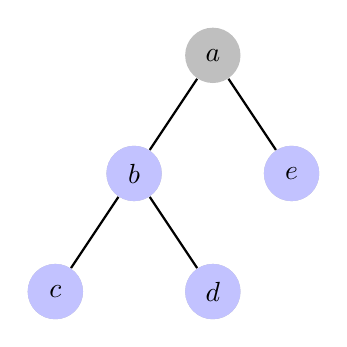
\begin{tikzpicture} [
                scale=1,
                vertex/.style={circle,fill=black!25,minimum size=20pt,inner sep=0pt},
                edge/.style = {draw,thick,-},
                selected vertex/.style = {vertex, fill=blue!24},
            ]
            \foreach \pos/\name in {
                    {(0,0)/c}, {(2,0)/d}, {(1,1.5)/b}, {(3,1.5)/e}, {(2,3)/a}}
                \node[vertex] (\name) at \pos {$\name$};
            \foreach \source/ \dest in {
                    b/c,b/d,a/b,a/e}
                \path[edge] (\source) edge (\dest);
            \foreach \vertex in {b,c,d,e}
                \path node[selected vertex] at (\vertex) {$\vertex$};
        \end{tikzpicture}
    \end{subfigure}
    \quad
    %%%%%%%%%%%%%%%%%%%%%%%%%%%%%%%%%%%%%%%%%%%%%%%%%%%%%%%%%%%%%%%%%%%%%%%%%%%%%%%%%%%%%
    \begin{subfigure}[b]{0.45\textwidth}
        \centering
        \caption{Sottografo (completo) indotto dai nodi dispari, e matching perfetto di costo minimo evidenziato}
        \label{fig:mchristmatching}
        \begin{tikzpicture} [
                scale=1,
                vertex/.style={circle,fill=black!25,minimum size=20pt,inner sep=0pt},
                edge/.style = {draw,thick,-},
                selected edge/.style = {draw,line width=5pt,-,blue!24},
            ]
            \foreach \pos/\name in {
                    {(0,0)/c}, {(2,0)/d}, {(1,1.5)/b}, {(3,1.5)/e}}
                \node[vertex] (\name) at \pos {$\name$};
            \foreach \source/ \dest in {
                    b/c,b/d,b/e,c/e,c/d,e/d}
                \path[edge] (\source) edge (\dest);
            \begin{pgfonlayer}{background}
                \foreach \source / \dest in {b/c,d/e}
                    \path[selected edge] (\source.center) -- (\dest.center);
            \end{pgfonlayer}
        \end{tikzpicture}
    \end{subfigure}
\end{figure}
    % \\[2pt]
% magic to split a figure https://tex.stackexchange.com/a/278748
\begin{figure}[htb]\ContinuedFloat
    \caption{Algoritmo di Christofides splittato in due pagine (cont.)}
    %%%%%%%%%%%%%%%%%%%%%%%%%%%%%%%%%%%%%%%%%%%%%%%%%%%%%%%%%%%%%%%%%%%%%%%%%%%%%%%%%%%%%
    \begin{subfigure}[b]{0.45\textwidth}
        \centering
        \caption{Ciclo Euleriano
            $ \langle c,b,d,e,a,b,c \rangle$
        }
        \label{fig:mchristeulertour}
        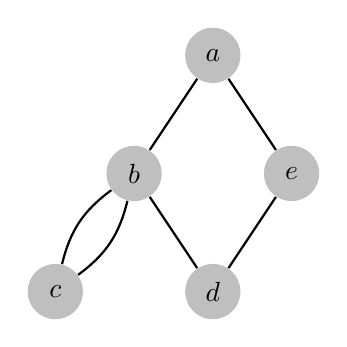
\begin{tikzpicture} [
                scale=1,
                vertex/.style={circle,fill=black!25,minimum size=20pt,inner sep=0pt},
                edge/.style = {draw,thick,-},
                bent right/.style = {bend right=20},
            ]
            \foreach \pos/\name in {
                    {(0,0)/c}, {(2,0)/d}, {(1,1.5)/b}, {(3,1.5)/e}, {(2,3)/a}}
                \node[vertex] (\name) at \pos {$\name$};
            \foreach \source/ \dest in {
                    b/d,a/b,a/e,d/e}
                \path[edge] (\source) edge (\dest);
            \foreach \source/ \dest in {
                    c/b,b/c}
                \path[edge] (\source) edge [bent right] (\dest);
        \end{tikzpicture}
    \end{subfigure}
    \quad
    %%%%%%%%%%%%%%%%%%%%%%%%%%%%%%%%%%%%%%%%%%%%%%%%%%%%%%%%%%%%%%%%%%%%%%%%%%%%%%%%%%%%%
    \begin{subfigure}[b]{0.45\textwidth}
        \centering
        \caption{Dopo lo \emph{shortcutting}:
            $ \langle c,b,d,e,a,\cancel{b},c \rangle$
        }
        \label{fig:mchristresult}
        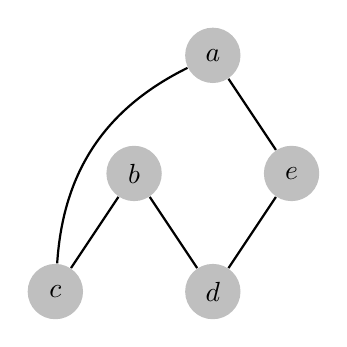
\begin{tikzpicture} [
                scale=1,
                vertex/.style={circle,fill=black!25,minimum size=20pt,inner sep=0pt},
                edge/.style = {draw,thick,-},
                bent right/.style = {bend right=30},
            ]
            \foreach \pos/\name in {
                    {(0,0)/c}, {(2,0)/d}, {(1,1.5)/b}, {(3,1.5)/e}, {(2,3)/a}}
                \node[vertex] (\name) at \pos {$\name$};
            \foreach \source/ \dest in {
                    b/d,a/e,d/e,b/c}
                \path[edge] (\source) edge (\dest);
            \foreach \source/ \dest in {
                    a/c}
                \path[edge] (\source) edge [bent right] (\dest);
        \end{tikzpicture}
    \end{subfigure}
\end{figure}

\lipsum{10}

\begin{figure}[h]
    \centering
    \caption{$3-CNF-SAT$ to $CLIQUE$}
    \label{fig:3cnfsatex}
    \begin{tikzpicture} [
            scale=1,
            vertex/.style={circle,fill=black!25,minimum size=20pt,inner sep=0pt},
            edge/.style = {draw,thin,-},
            outbound edge/.style = {draw,line width=4pt,-,blue!30},
            selected edge/.style = {draw,line width=4pt,-,red!30},
        ]
        % First we draw the vertices
        \foreach \pos/\name/\label in {
                % top left
                {(-1.5,5)/c/x_3},
                {(-2.5,3.5)/b/x_2},
                {(-3.5,2)/a/\bar{x_1}},
                % top right
                {(1.5,5)/d/x_1},
                {(2.5,3.5)/e/x_2},
                {(3.5,2)/f/\bar{x_3}},
                % bottom row
                {(2,0)/g/\bar{x_3}},
                {(0,0)/h/\bar{x_2}},
                {(-2,0)/i/x_1}}
            \node[vertex] (\name) at \pos {\name $\label$};
        % Connect vertices with edges
        \foreach \source/ \dest in {
                f/g,f/i,
                e/g,e/i,
                d/g,d/h,d/i,
                c/d,c/e,c/h,c/i,
                b/d,b/e,b/f,b/g,b/i,
                a/e,a/f,a/g,a/h}
            \path[edge] (\source) -- (\dest);
        % color some edges on background layer
        \begin{pgfonlayer}{background}
            \foreach \source / \dest in {c/d,d/i,i/c}
                \path[outbound edge] (\source.center) -- (\dest.center);
            \foreach \source / \dest in {a/e,e/g,g/a}
                \path[selected edge] (\source.center) -- (\dest.center);
        \end{pgfonlayer}
    \end{tikzpicture}
\end{figure}

\subsection{Parole in libertà}

Tutte le parole accentate si possono estrarre con

\texttt{grep -rEiohI '[a-z]*(à|è|é|ì|ò|ù)' | sort -u}

\begin{itemize}[noitemsep,parsep=0pt,partopsep=0pt,topsep=0pt]
    \item \texttt{-r}:
        Read all files under each directory, recursively
    \item \texttt{-E}:
        Interpret PATTERN as an extended regular expression
    \item \texttt{-i}:
        Ignore case distinctions in both the PATTERN and the input files
    \item \texttt{-o}:
        Print only the matched (non-empty) parts of a matching line
    \item \texttt{-h}:
        Suppress the prefixing of file names on output
    \item \texttt{-I}:
        Process a binary file as if it did not contain matching data
    \item \texttt{sort -u}:
        Sort the output and remove duplicates
\end{itemize}

Le parole servono in modo che l'autocomplete le veda e le suggerisca:

affidabilità
andrà
associatività
avrà
Bé
biiettività
capacità
cardinalità
cioè
complessità
Complessità
così
difficoltà
Difficoltà
divisibilità
Divisibilità
dovrà
è
È
facilità
farà
finché
generalità
già
identità
Identità
inapprossimabilità
Inapprossimabilità
leggibilità
libertà
massimalità
metà
molteplicità
né
necessità
ottimalità
perché
Perché
però
più
polinomialità
potrà
primalità
probabilità
Probabilità
proprietà
Proprietà
pseudoprimalità
può
Può
qualità
quantità
randomicità
realtà
Riducibilità
sarà
sé
segnerà
Sì
soddisfacibilità
Soddisfacibilità
suriettività
transitività
unicità
Unicità
unità
utilità
validità
velocità
verità


\begin{figure}[h]
    \centering
    \caption{Unweighted graph}
    \label{fig:ug2}
    \begin{tikzpicture} [
            auto,
            swap,
            scale=1.4,
            vertex/.style={circle,fill=black!25,minimum size=20pt,inner sep=0pt},
            selected vertex/.style = {vertex, fill=red!24},
            edge/.style = {draw,thick,-},
            weight/.style = {font=\small},
            selected edge/.style = {draw,line width=5pt,-,red!50},
            outbound edge/.style = {draw,line width=5pt,-,blue!50},
            ignored edge/.style = {draw,line width=5pt,-,black!20}
        ]
        % First we draw the vertices
        \foreach \pos/\name in {
                {(0,0)/A},
                {(0,2)/B},
                {(2,2)/C},
                {(4,2)/D},
                {(2,0)/E}}
            \node[vertex] (\name) at \pos {$\name$};
        % Connect vertices with edges and draw weights
        \foreach \source/ \dest in {
                B/C, C/E, C/D, D/E}
            \path[edge] (\source) -- (\dest);
        % color a node
        % \foreach \vertex in {B, D, E}
            % \path node[selected vertex] at (\vertex) {$\vertex$};
        \begin{pgfonlayer}{background}
            % \foreach \source / \dest in {B/C}
                % \path[outbound edge] (\source.center) -- (\dest.center);
            % \foreach \source / \dest in {D/G}
                % \path[selected edge] (\source.center) -- (\dest.center);
            % \foreach \source / \dest in {F/D}
                % \path[ignored edge] (\source.center) -- (\dest.center);
        \end{pgfonlayer}
    \end{tikzpicture}
\end{figure}


